%----------------------------------------------------------------------------
%bb defines the bounding box for the pdf
%viewport defines the area of the pdf used
%in sidewaysfigure the last entry in bb moves the caption toward/away the pic
%in sidewaysfigure the second entry in bb moves the pic toward/away the caption
%----------------------------------------------------------------------------
\begin{figure}
\scalebox{0.6}[0.6]{
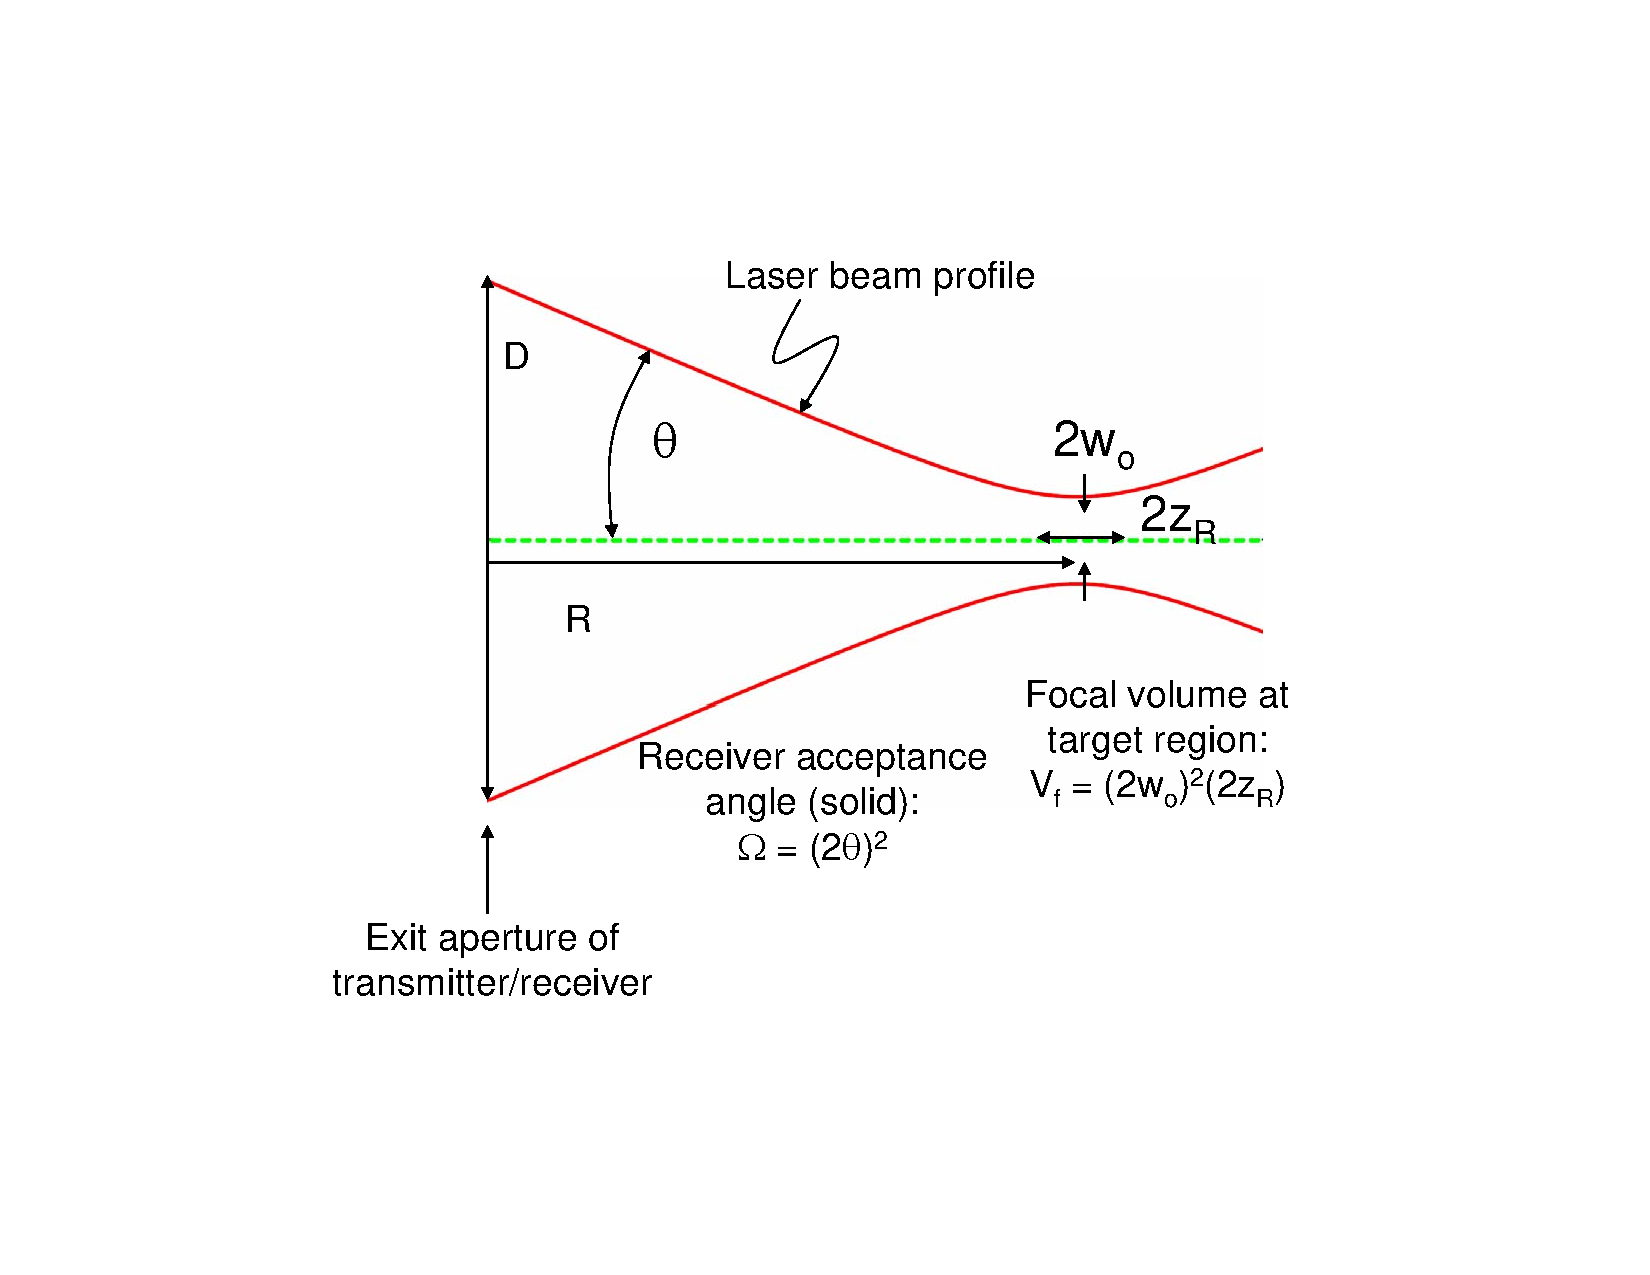
\includegraphics[bb=35 125 489 480]
{backscatter_figure/backscatter_figure.pdf}
}
\caption[Backscatter geometry]{Backscatter geometry. After leaving the exit aperture of diameter D, a laser beam is brought to a focus a distance R from the aperture. The dimensions of the focal volume and the far-field divergence ($\theta$) depend only on D, R, and the laser wavelength $\lambda$.}
\label{backscatter_figure}
\end{figure}
%----------------------------------------------------------------------------
